
\documentclass[a4paper,12pt]{article} % добавить leqno в [] для нумерации слева

\usepackage[left=2cm,right=2cm,
top=2cm,bottom=2cm,bindingoffset=0cm]{geometry}

\usepackage{amsmath,amsfonts,amssymb,amsthm,mathtools} % AMS
\usepackage{icomma} 
\mathtoolsset{showonlyrefs=true} % Показывать номера только у тех формул, на которые есть \eqref{} в тексте.
\usepackage{euscript}	 % Шрифт Евклид
\usepackage{mathrsfs} % Красивый матшрифт
\usepackage{enumitem}
\usepackage{siunitx}
\usepackage{tikz} % To generate the plot from csv
\usepackage{pgfplots}

%%% Заголовок
\author{Kseniia Kasianova}
\title{Macroeconomics. Homework 1}
\date{\today}

\newcommand{\latinword}[1]{\textsf{\itshape #1}}%

\begin{document}

{\color{blue} \latinword{Begin to write your assignment here}}

\noindent\makebox[\linewidth]{\rule{\textwidth}{0.4pt}}


\section*{Test 1}
\subsection*{Problem 1}

\begin{enumerate}[label=\alph*)]
	\item 
The equation of a consumption function, where consumption depends on disposable income and interest rate:
\[  C=C_0+MPC(Y-T) - b \cdot r  \] 
where $ MPC = \frac{\partial C}{\partial Y} $ is marginal propensity to consume and $ b = \frac{\partial C}{\partial r} $ is marginal propensity to consume influenced by an interest rate.   

\item  The equation of a consumption function, where consumption depends only on disposable
income, taxes have a fixed part $ T_{0} $ and a part proportionate to the global income of the economy:
\[  C=C_0+MPC(Y-T_{0}-t \cdot Y)  \]

\item  The equation of an investment function:
 \[ I=I_{0}-d \cdot r \] 
 where $ I $ is investment function; $ I_{0} $ is autonomous investment, which is independent of the level of income (income inelastic) part of investment influenced by exogenous factors, like innovations, growth of population or shocks; $ d $  is marginal investment rate, that characterizes elasticity of investment demand; $ r $ is an interest rate.     
 
\item  A balanced market of goods and services: 
\begin{gather*}
\bar{Y} = F(\bar{K},\bar{L})\\
C=C_0+MPC(Y-T_{0}-t \cdot Y) \\
I=I_{0}-d \cdot r\\
G=\bar{G}
\end{gather*}
Using an equation for balanced market of a closed economy $ Y=C+I+G $, we get: 
\begin{gather*}
Y=C_0+MPC(Y-T_{0}-t\cdot Y) + I_{0}-d \cdot r + \bar{G}\\
Y-MPC(Y-tY)=C_0-MPC \cdot T_{0} + I_{0}-d\cdot r + \bar{G}\\
Y=\dfrac{C_0+ I_{0}-MPC \cdot T_{0} -d\cdot r + \bar{G}}{1-MPC+MPC\cdot t}
\end{gather*}

\item  The budget multiplier for this economy is $ \dfrac{\partial Y}{\partial G} = \dfrac{1}{1-MPC+MPC\cdot t} $ and  the …fiscal multiplier is $ \dfrac{\partial Y}{\partial T} = -\dfrac{MPC}{1-MPC+MPC\cdot t} $

\item  In this economy $ MPC=0.65, MPS=0.35, t=0.1 $, the budget multiplier is $ \dfrac{\partial Y}{\partial G} = \dfrac{1}{1-0.65+0.65\cdot 0.1} \approx 2.41 $, the …fiscal multiplier is $ \dfrac{\partial Y}{\partial T} = -\dfrac{0.65}{1-0.65+0.65\cdot 0.1} \approx 1.57  $

\end{enumerate}

\subsection*{Problem 2} 

In the following economy consumption function is: $ C = c \cdot Y +C_{0}  = 0.8Y + 50 $; autonomous
investment is  $ I_{0} = 10 $.

\begin{enumerate}[label=\alph*)]
	 

\item Plotting consumption and spending regarding to income, we have:

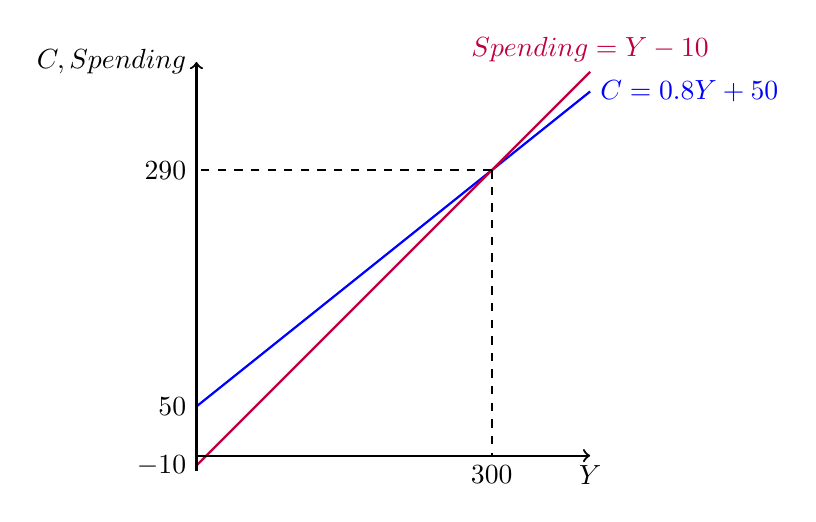
\begin{tikzpicture}[domain=0:5,scale=1,thick]
\usetikzlibrary{calc}   %allows coordinate calculations.

%Define linear parameters 
\def\dint{0.625}        %Y-intercept for DEMAND.
\def\dslp{0.8}         %Slope for DEMAND.
\def\sint{-0.125}          %Y-intercept for SUPPLY.
\def\sslp{1}          %Slope for SUPPLY.
\def\demand{\x,{\dslp*\x+\dint}}
\def\supply{\x,{\sslp*\x+\sint}}

% Define coordinates
\coordinate (pfq) at  (3.75,0);
\coordinate (pfp) at  (3.75,3.625);
\coordinate (sfq) at  (0,3.625);

% DEMAND
\draw[thick,color=blue] plot (\demand) node[right] {$C = 0.8Y+50$};

% SUPPLY
\draw[thick,color=purple] plot (\supply) node[above] {$ Spending = Y-10 $};

% Draw axes, and dotted equilibrium lines.
\draw[->] (0,0) -- (5,0) node[below] {$Y$};
\draw[->] (0,-0.2) -- (0,5) node[left] {$C, Spending$};

%Price floor and ceiling lines
\draw[dashed] (pfp) -- (pfq) node[below] {$300$};
\draw[dashed] (pfp) -- (sfq) node[left] {$290$};
\node [left] at (0,0.625) {$ 50 $};
\node [left] at (0,-0.125) {$ -10 $};

\end{tikzpicture}

The balanced value for income can be also found algebraically. We know, that $ Y = C + I +G + Nx $, which equals $ Y = C + I  $ , since in our economy $ G=0, Nx=0 $. We also know, that $ Spending = Y - I = Y - 10 $ and $ C =  c \cdot Y +C_{0}  = 0.8Y + 50  $. Combining that we get: 
\begin{gather*}
 Y - I=C\\
 Y - 10 = 0.8Y + 50 \\
 0.2Y=60\\
 Y=300
\end{gather*}

\item We know, that $ I=10 $ and $ S = Y-C=Y-( 0.8Y + 50)=0.2Y-50 $ Plotting the investment and the savings function on the same graph, we can see: 

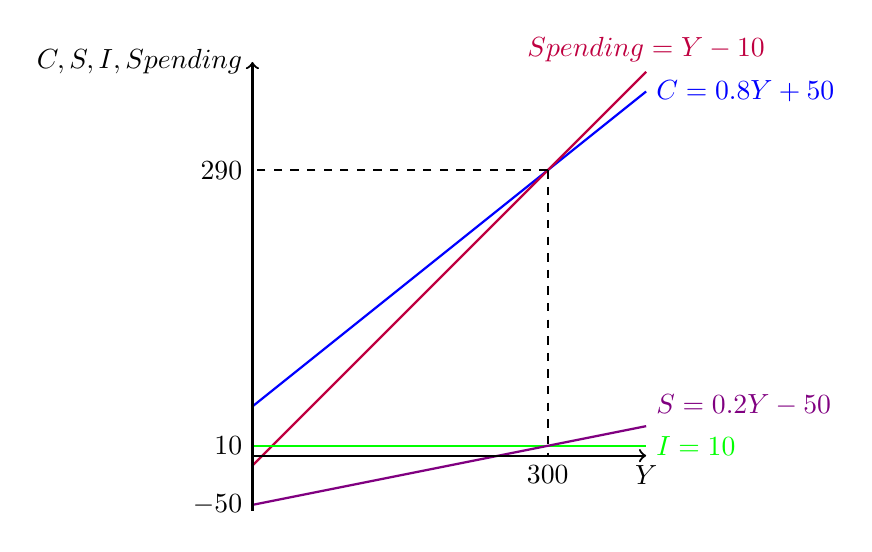
\begin{tikzpicture}[domain=0:5,scale=1,thick]
\usetikzlibrary{calc}   %allows coordinate calculations.

%Define linear parameters for supply and demand
\def\dint{0.625}          %Y-intercept for DEMAND.
\def\dslp{0.8}         %Slope for DEMAND.
\def\sint{-0.125}          %Y-intercept for SUPPLY.
\def\sslp{1}          %Slope for SUPPLY.
\def\inin{0.125} %int for I
\def\sain{-0.625} 
\def\saslp{0.2}

\def\demand{\x,{\dslp*\x+\dint}}
\def\supply{\x,{\sslp*\x+\sint}}
\def\invest{\x,{\inin}}
\def\savin{\x,{\saslp*\x+\sain}}

% Define coordinates.
\coordinate (pfq) at  (3.75,0);
\coordinate (pfp) at  (3.75,3.625);
\coordinate (sfq) at  (0,3.625);

\draw[thick,color=blue] plot (\demand) node[right] {$C = 0.8Y+50$};
\draw[thick,color=purple] plot (\supply) node[above] {$ Spending = Y-10 $};
\draw[thick,color=green] plot (\invest) node[right] {$ I = 10 $};
\draw[thick,color=violet] plot (\savin) node[above right] {$ S = 0.2Y-50 $};


% Draw axes, and dotted equilibrium lines.
\draw[->] (0,0) -- (5,0) node[below] {$Y$};
\draw[->] (0,-0.7) -- (0,5) node[left] {$C,  S, I, Spending$};

%Price floor and ceiling lines
\draw[dashed] (pfp) -- (pfq) node[below] {$300$};
\draw[dashed] (pfp) -- (sfq) node[left] {$290$};
\node [left] at (0,-0.625) {$ -50 $};
\node [left] at (0,0.125) {$ 10 $};

\end{tikzpicture}

The point
of intersection between these two curves $ S $ and $ I $ shows us, that with $ S-I=0 $, while $ Nx=0 $ we have a balanced economy. This happens because when we are to the right of that point the supply for investment is higher than the demand, so there is a deflationary gap on the investment market. Similarly, to the left of equilibrium point the demand for investment is higher, so there is an inflationary gap. Both of these gaps influence motivation mechanisms, which stimulate  economic agents to act in such a way, that leads the economy to equilibrium. 

  $ C + S $ is disposable income line, and since in our economy $S=I  $ we can derive it by  shifting the consumption function upward by 10.  

\item The inclusion of investment expenditures to those of consumption increases the value for balanced income: 


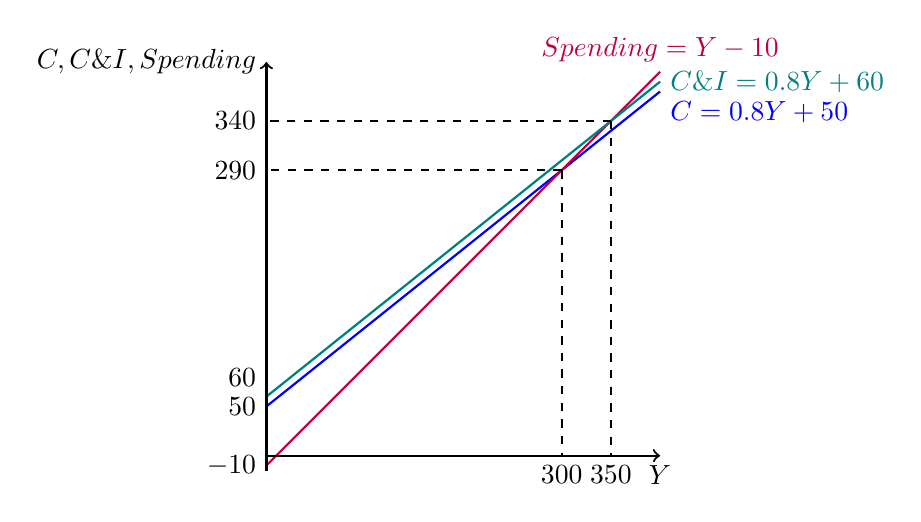
\begin{tikzpicture}[domain=0:5,scale=1,thick]
\usetikzlibrary{calc}   %allows coordinate calculations.

%Define linear parameters 
\def\dint{0.625}        %Y-intercept for DEMAND.
\def\dslp{0.8}         %Slope for DEMAND.
\def\sint{-0.125}          %Y-intercept for SUPPLY.
\def\sslp{1}          %Slope for SUPPLY.
\def\ciin{0.75}


\def\demand{\x,{\dslp*\x+\dint}}
\def\supply{\x,{\sslp*\x+\sint}}
\def\candi{\x,{\dslp*\x+\ciin}}


% Define coordinates
\coordinate (pfq) at  (3.75,0);
\coordinate (pfp) at  (3.75,3.625);
\coordinate (sfq) at  (0,3.625);
\coordinate (qqq) at  (4.375,4.25);
\coordinate (qqx) at  (4.375,0);
\coordinate (qqy) at  (0,4.25);

% DEMAND
\draw[thick,color=blue] plot (\demand) node[below right] {$C=0.8Y+50$};

% SUPPLY
\draw[thick,color=purple] plot (\supply) node[above] {$ Spending = Y-10 $};

\draw[thick,color=teal] plot (\candi) node[right] {$C \& I = 0.8Y+60$};


% Draw axes, and dotted equilibrium lines.
\draw[->] (0,0) -- (5,0) node[below] {$Y$};
\draw[->] (0,-0.2) -- (0,5) node[left] {$C, C \& I, Spending$};

%Price floor and ceiling lines
\draw[dashed] (pfp) -- (pfq) node[below] {$300$};
\draw[dashed] (pfp) -- (sfq) node[left] {$290$};

\draw[dashed] (qqq) -- (qqx) node[below] {$350$};
\draw[dashed] (qqq) -- (qqy) node[left] {$340$};

\node [above left] at (0,0.75) {$ 60 $};
\node [left] at (0,0.625) {$ 50 $};
\node [left] at (0,-0.125) {$ -10 $};

\end{tikzpicture}


To find the value of the investment multiplier we should use the equation for the balanced market $ Y=C_{0}+MPC\cdot Y + I $, using which we have: 
\begin{gather*}
Y=\dfrac{C_{0}+I}{1-MPC}\\
 \dfrac{\partial Y}{\partial I} = \dfrac{1}{1-MPC} = \dfrac{1}{1-0.8} = 5
 \end{gather*}
The value of the investment multiplier in this economy equals inverse of $ MPS  $, which means the higher is marginal propensity to save, the lower is the demand for investment. 


\end{enumerate}


\subsection*{Problem 3}

 We have a closed economy consisting of three classes of agents: households, …firms and
the government, operating on different markets. Prices and wages are perfectly flexible, public spending is exogenous and money is controlled exclusively by the government. The government …finances its
expenditures through debt or money creation. 


\begin{enumerate}[label=\alph*)]


\item  Agents in this economy operate on three different markets: labor market, good market and money market.    

Labor market is    such a part of the economy, where  the equilibrium level of employment and equilibrium wage are derived through the supply and demand mechanisms  as a result of competition between economic agents. It is           described in this economy by the following equations: 


\begin{itemize}
\item $ N^{s} = 0.04 \times (\frac{W}{P})^{2} $ is  the function of labor supply, where $ \frac{W}{P} $ is the real wage 
\item $ N^{d}= 400 \times (\frac{W}{P})^{-2} $ is  the labor demand 
\item $  N^{s} = N^{d} = N $
\item  $ LF = 6 $ is the labor force measured in millions
\end{itemize}




Good market (or real market)  is   the  form of competitive economic relations between economic agents regarding sale and purchase of all the end-use goods and services produced in the economy during a certain period of time. It is described in this economy by the following equations: 
 
 \begin{itemize}
 	\item $ Y = 40 \sqrt{N} $ is the output, where  N is the level of employment (in million)
 	\item $ S = 800r -40 $ is the household savings, where  r  is the real interest rate
 	\item $  I = -200r + 50$ is  the business investment 
 	\item $ G = 10 $ is  the government spending 
 	\item $  C = Y - S $ is the consumption
 \end{itemize}
 

 
 Money market is  the part of financial market where the demand and supply of money determine the interest rate and the "price" of money. It is described in this economy by the following equations: 
 
 
  \begin{itemize}
 	\item $ M^{s} =  160 $ is  the money supply function
 	\item $ M^{d} = 0.5PY $ is the money demand function
 	\item $  M^{s} = M^{d} = M $ is  the government spending 
 \end{itemize}
 


The model of this economy is inspired by the Classical school, because prices and wages are considered to be flexible, since all of the markets regulate themselves and operate efficiently without government intervention.

\item  In this economy exogenous variables are labor force, government spending, net export, money supply, autonomous investment, autonomous consumption, marginal propensity to consume, etc.; endogenous variables are output, labor supply, labor demand,  level of employment, real wage, household savings, business investment, consumption, real interest rate, money demand, general price level.

\item  To determine the set of variables we start with finding equilibrium on labor market: 
\begin{gather*}
  N^{s} = N^{d} = N  \\
0.04 \times \left( \frac{W}{P}\right) ^{2}  = 400 \times \left( \frac{W}{P}\right) ^{-2}  \\
\left( \frac{W}{P}\right) ^{4} = 10000  \\
 \left( \frac{W}{P}\right) = 10 \Rightarrow N=4 \Rightarrow Y=80
\end{gather*}
On the good market we have: 
\begin{gather*}
S=I+G\\
 800r -40 =  -200r + 50 + 10  \\
  1000r=100  \Rightarrow  r=0.1\\
  S = 800 \times 0.1 - 40 = 40 \\
  I = -200 \times 0.1 + 50 = 30 \\
  C = 80 - 40 = 40 
\end{gather*}

On the money market:
\begin{gather*}
M^{s} = M^{d} = M \\
 160  = 0.5P \times 80 \Rightarrow P = 4  
\end{gather*}

Since we know that $ LF = 6 $ , we can describe the employment situation by counting unemployment rate:
\[ U = \dfrac{LF - N}{LF} = \dfrac{6-4}{6}= \dfrac{1}{3}\approx 0.33\]

\item  The government …fix a minimum for the real wage at a value of 12. The consequences are the following: 
  	
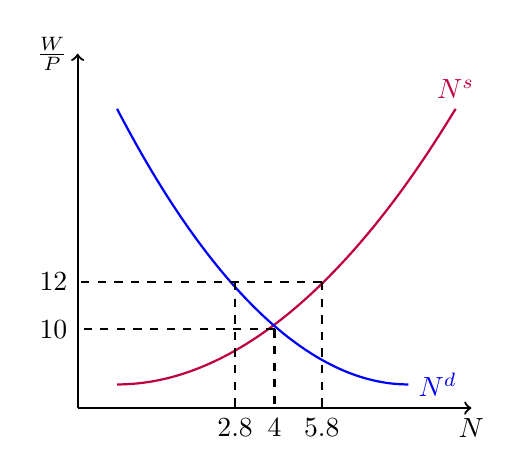
\begin{tikzpicture}[domain=0:5,scale=1,thick]
\usetikzlibrary{calc}   %allows coordinate calculations.

%Define linear parameters for supply and demand
\coordinate (a) at (3.1,1.6);
\coordinate (b) at (0,1.6);
\coordinate (c) at (2.5,1);
\coordinate (d) at (0,1);
\coordinate (f) at (3.1,0);
\coordinate (g) at (2.5,0);
\coordinate (h) at (2,1.6);
\coordinate (i) at (2,0);


\draw[thick,color=purple] (0.5,0.3) coordinate (NS1) parabola (4.8,3.8) coordinate (NS2) node[above] {$ N^{s} $} ;
\draw[thick,color=blue] (0.5,3.8) coordinate (ND1) parabola[bend at end] (4.2,0.3) coordinate (ND2) node[right] {$ N^{d} $};


% Draw axes, and dotted equilibrium lines.
\draw[->] (0,0) -- (5,0) node[below] {$N$};
\draw[->] (0,0) -- (0,4.5) node[left] {$ \frac{W}{P} $};

%Price floor and ceiling lines
\draw[dashed] (a) -- (b) node[left] {$12$};
\draw[dashed] (c) -- (d) node[left] {$10$};
\draw[dashed] (a) -- (f) node[below] {$5.8$};
\draw[dashed] (c) -- (g) node[below] {$4$};
\draw[dashed] (h) -- (i) node[below] {$2.8$};

\end{tikzpicture}

Now the labor supply exceeds labor demand $ N^{s} - N^{d} = 0.04 \times 12^{2} - 400 \times 12^{-2} \approx 5.8 -2.8 = 3 $ and new unemployment rate equals to $ U = \dfrac{LF - N^{d}}{LF} = \dfrac{6-3}{6}= 0.5$, which is higher than it was before government intervention.


\item  Wishing to reduce unemployment, the government decides to increase the public spending $ \bigtriangleup G = 5 $.  
So to understand, how fiscal policy influenced the output, we need IS-LM model. 
In this model, LM function does not depend on real interest rate (note that $ P $ has not changed):
\begin{gather*}
\dfrac{M^{d}}{P} = \dfrac{M^{s}}{P} \\
\dfrac{0.5PY}{P} = \dfrac{160}{P} \\
Y=\dfrac{320}{P} = \dfrac{320}{4} = 80
\end{gather*}
While IS function does not depend on the output: 
\begin{gather*}
Y = C + I + G \\
Y = Y - S + I + G \\
Y = Y - 800r + 40  -200r + 50 + 10   \Rightarrow  r=0.1
 \end{gather*}
Because of government intervention IS shifts up, so we see the following result:
\begin{gather*}
Y = Y - 800r + 40  -200r + 50 + 15   \Rightarrow  r'=0.105 
\end{gather*}


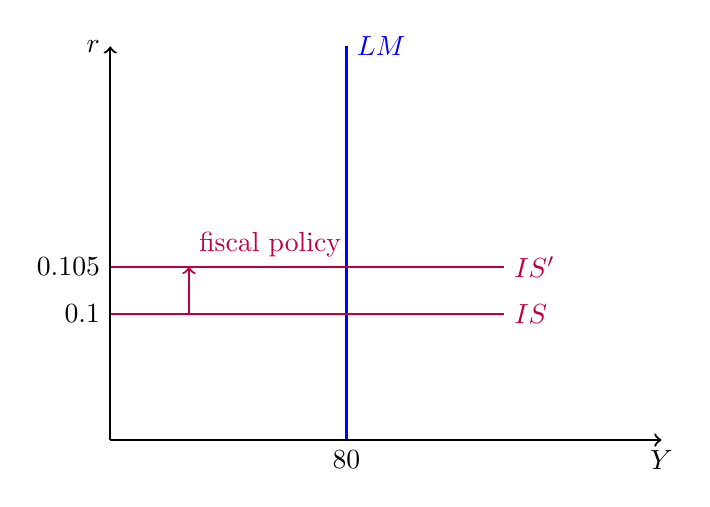
\begin{tikzpicture}[domain=0:5,scale=1,thick]
\usetikzlibrary{calc}   %allows coordinate calculations.


\draw[thick,color=blue] (3,0) -- (3,5) node[right] {$ LM $};

\draw[thick,color=purple] (0,2.2) -- (5,2.2) node[right] {$ IS' $};
\draw[thick,color=purple] (0,1.6) -- (5,1.6) node[right] {$ IS $};


% Draw axes, and dotted equilibrium lines.
\draw[->] (0,0) -- (7,0) node[below] {$Y$};
\draw[->] (0,0) -- (0,5) node[left] {$r$};

\draw[->, color=purple] (1,1.6) -- (1,2.2) node[above right] {fiscal policy};


\node [below] at (3,0) {$ 80 $};
\node [left] at (0,2.2) {$ 0.105 $};
\node [left] at (0,1.6) {$ 0.1 $};


\end{tikzpicture}

New equilibrium in IS-LM shown on the plot leaves us with higher interest rate, while  output stays the same. Level of employment and unemployment also stay the same,  household savings  
$ S' = 800 \times 0.105 - 40 = 44  \Rightarrow \bigtriangleup S=4 $ increase by 4, investment 
$ I' = -200 \times 0.105 + 50 = 29  \Rightarrow \bigtriangleup I=-1 $ decrease by 1. These results show us, that in this economy fiscal policy would be ineffective  for unemployment reduction.


\item  Noting the consequences of borrowing, the government decide to increase the supply of money
$ \bigtriangleup M^{s} = 5 $. In this situation LM function shifts right to the right:
\begin{gather*}
\dfrac{M^{d}}{P} = \dfrac{M^{s}}{P} \\
\dfrac{0.5PY}{P} = \dfrac{165}{P} \\
Y'=\dfrac{330}{P} = \dfrac{330}{4} = 82.5
\end{gather*}


With new equilibrium in IS-LM shown on the plot we have the same interest rate, but and 2.5 increase in output: 

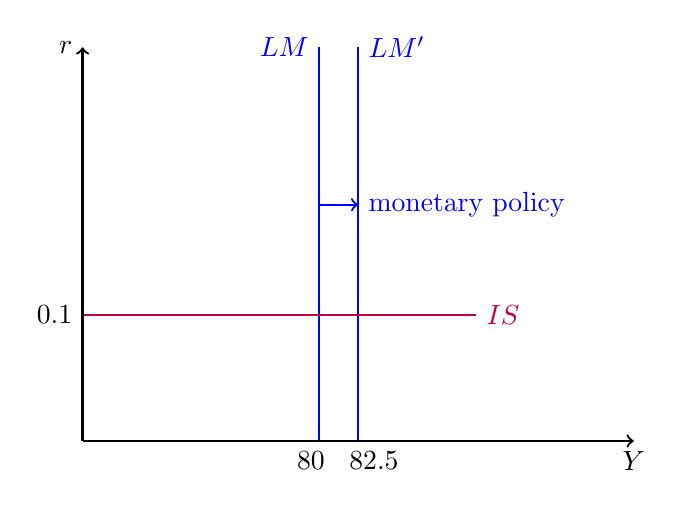
\begin{tikzpicture}[domain=0:5,scale=1,thick]
\usetikzlibrary{calc}   %allows coordinate calculations.

\draw[thick,color=blue] (3,0) -- (3,5) node[left] {$ LM $};

\draw[thick,color=blue] (3.5,0) -- (3.5,5) node[right] {$ LM' $};

\draw[thick,color=purple] (0,1.6) -- (5,1.6) node[right] {$ IS $};


% Draw axes, and dotted equilibrium lines.
\draw[->] (0,0) -- (7,0) node[below] {$Y$};
\draw[->] (0,0) -- (0,5) node[left] {$r$};

\draw[->, color=blue] (3,3) -- (3.5,3) node[right] {monetary policy};

\node [below] at (2.9,0) {$ 80 $};

\node [below] at (3.7,0) {$ 82.5 $};
\node [left] at (0,1.6) {$ 0.1 $};



\end{tikzpicture}

Household savings and investment stay the same, consumption increase by 2.5.  
New level of employment $ N = \dfrac{Y^{2}}{1600} \approx 4.25  $  is 0.25 mln higher, than before the intervention. We can assume, that labor force has not changed, so we have a new level of unemployment $ U = \dfrac{LF - N}{LF} = \dfrac{6-4.25}{6}= \dfrac{1}{3}\approx 0.29$ , which is $ 4\% $ less, than before the monetary policy.
 This  shows us, that in this economy monetary policy would be more effective, than fiscal  for unemployment reduction.



\end{enumerate}

\end{document}